% =====================================================================
% Bias-corrected estimation of the interventional outcome density under
% a continuous, multidimensional treatment, with an MCD nuisance.
%
% Notation follows the companion MCD paper:
%   mixture ratio        pi          (\ratio)
%   contrast function    D_pi        (\contrast)
%   density ratio        R           (\DensityRatio)
%   augmented pair       (W,Z),  W=(T,X,Y)
%   densities            f_{...}     (\pf{...})
% The generalized propensity score is written e(t|x) to avoid colliding
% with the mixture ratio; the score displacement of the classifier is
% written S(w;beta) to avoid colliding with the contrast function.
% =====================================================================

\documentclass[11pt]{article}
\usepackage[T1]{fontenc}
\usepackage[margin=1in]{geometry}
\usepackage{amsmath,amssymb,amsthm}
\usepackage{bm}
\usepackage{relsize}
\usepackage{dsfont}
\usepackage{mathtools}
\usepackage{hyperref}
\usepackage[round]{natbib}
\usepackage{parskip}
\usepackage{booktabs}
\usepackage{array}
\usepackage{algorithm}
\usepackage{algpseudocode}

\theoremstyle{plain}
\newtheorem{theorem}{Theorem}
\newtheorem{mypropo}{Proposition}
\newtheorem{lem}{Lemma}
\newtheorem{corollary}{Corollary}
\theoremstyle{definition}
\newtheorem{mydef}{Definition}
\newtheorem{assumption}{Assumption}
\theoremstyle{remark}
\newtheorem{remark}{Remark}

% ---- subset of 00_Notations.tex ----
\newcommand{\ourmethod}{\text{MCD}\,}
\newcommand{\mcd}{\text{MCD}\,}
\newcommand{\MCF}{\ensuremath{\text{MCFunct}}}
\newcommand{\MDC}{\ensuremath{\text{MDCond}}}
\newcommand{\pE}{\ensuremath{\mathbb{E}}}
\newcommand{\pP}{\ensuremath{\mathbb{P}}}
\newcommand{\Var}{\mathbb{V}\text{ar}}
\newcommand{\R}{\mathbb{R}}
\newcommand{\cW}{\ensuremath{\mathcal{W}}}
\newcommand{\cX}{\ensuremath{\mathcal{X}}}
\newcommand{\cY}{\ensuremath{\mathcal{Y}}}
\newcommand{\cT}{\ensuremath{\mathcal{T}}}
\newcommand{\cR}{\ensuremath{\mathcal{R}}}
\newcommand{\pf}[1]{\ensuremath{\,\mathlarger{\textit{f}}_{#1}}}
\newcommand{\pfhat}[1]{\ensuremath{\,\mathlarger{\widehat{\textit{f}}}_{#1}}}
\newcommand{\ratio}{\ensuremath{\pi}}
\newcommand{\contrast}{D_{\ratio}}
\newcommand{\contrasthat}{\widehat{D}_{\mcd}}
\newcommand{\DensityRatio}{\text{R}}
\newcommand{\mDwz}[1]{\ensuremath{\mathcal{D}}_{#1}^{W,Z}}
\newcommand{\betahat}{\widehat{\beta}}
\newcommand{\Indi}{\ensuremath{\mathds{1}}}
\newcommand{\ks}{k}
\newcommand{\cO}{\mathcal{O}}
% ---- specific to this paper ----
\newcommand{\dd}{\,\mathrm{d}}
\newcommand{\IF}{\mathrm{IF}}
\newcommand{\gps}{e}
\newcommand{\score}{S}
\newcommand{\Rem}{\mathrm{Rem}}

\usepackage{tikz}
\usetikzlibrary{positioning, arrows.meta}
\tikzset{
    dagnode/.style={circle, draw, thick, minimum size=1cm},
    dagarrow/.style={-{Latex[length=3mm,width=2mm]}, thick}
}

\title{Bias-Corrected Estimation of the Interventional Density\\
Under a Continuous, Multidimensional Treatment}
\author{}
\date{}

\begin{document}
\maketitle

\begin{abstract}
We study the estimation of the interventional density of a scalar outcome under a
continuous, possibly multidimensional treatment. Under the backdoor adjustment, this
 reduces to a
conditional density problem whose conditioning set contains the treatment and all
confounders. Marginal contrastive discrimination is well suited to this high-dimensional
conditioning set, as it replaces the conditional density by a univariate marginal and a
binary classifier. The resulting plug-in estimator, however, inherits a first-order bias.

Removing this bias by the standard one-step correction requires the influence function of
the target, which involves the generalized propensity score --- a conditional density in
the treatment, and precisely the object the contrastive construction was meant to avoid.
Our main contribution is to re-express this correction through the contrastive
factorization itself. The generalized propensity score then disappears,but in exchange, the correction
now requires the influence function of the fitted contrast function. 


\end{abstract}

\section{Introduction}
\label{sec:intro}

A prediction describes what is likely to happen; a causal statement describes what would
happen under an intervention. Decisions call for the second. A clinician choosing a dose,
a regulator setting an exposure limit, and an analyst evaluating a policy all need the
distribution of an outcome under an intervention. Randomized experiments answer such questions
by construction, but they are often unavailable, and the causal quantity must then be
recovered from observational data, in which the treatment is chosen rather than assigned
and the reasons for the choice usually affect the outcome as well.

Most work reports a mean: the average treatment effect, or, for a treatment ranging over
a continuum, the dose-response curve $t \mapsto \pE[Y(t)]$, where $Y(t)$ is the potential
outcome under treatment level $t$. A mean, however, collapses a distribution to a single
number, and two interventions with equal means may induce very different distributions of
the outcome. Whenever the question concerns the probability of exceeding a threshold, the
spread of the response, or any functional of the outcome law beyond its first moment, the
relevant object is the full interventional density
\[
p_t(y) = \pf{Y(t)}(y),
\]
the density of $Y(t)$ at the point $y$. Its semiparametric theory was developed by
\citet{kennedy2023density}, who derived the efficient influence function and a doubly
robust estimator, with further estimators due to \citet{melnychuk2023flows},
\citet{ham2024logconcave} and \citet{martinez2023stein}. All of these assume a treatment
with finitely many levels.

We treat the continuous case, which is both more common in applications and harder in
theory. Doses, durations, concentrations and continuous policy instruments are not
naturally discretized, and applications often involve several such quantities at once, so
the treatment is a vector $T \in \cT \subseteq \R^d$. With a continuous treatment the
propensity score becomes the generalized propensity score of \citet{imbens2000} and
\citet{hirano2004}, a conditional density in $t$ rather than a probability, and the
target is no longer estimable at the parametric rate: \citet{kennedy2017continuous} showed
that the dose-response curve requires smoothing in the treatment argument, and
\citet{colangelo2020} gave the corresponding debiased machine learning estimator. In this
line of work the target has remained the mean; we take it to be the density.

Our identification is the backdoor adjustment \citep{pearl1995,pearl2009}, which writes
the target as the conditional outcome density averaged over the covariates,
\[
p_t(y) = \pE_X\big[\pf{Y \mid T=t,X}(y)\big].
\]
Estimation therefore reduces to a single conditional density, evaluated at the treatment
level $t$ and averaged over the covariate distribution. This conditional density is where
the difficulty concentrates: its conditioning set is the pair $(T,X)$, which holds the
treatment and every confounder and is high-dimensional, while the outcome is scalar.
Standard nonparametric estimators are ill suited to this setting, since their rates
deteriorate with the dimension of the conditioning argument
\citep{stone1980,Tsybakov2009NonparametricEstimation}, and this rate governs the error of
the whole procedure.

Marginal contrastive discrimination \citep{meziani2025mcd} is built for this particular setting.
It writes the conditional density as a univariate marginal times a density ratio, and
estimates the ratio by a binary classifier that separates observed vectors from vectors
whose outcome has been resampled from its own marginal. No density on a high-dimensional
space is ever fitted: the marginal is univariate and the ratio is obtained by
classification, a problem any supervised learner can solve. The same principle drives
noise-contrastive estimation \citep{gutmann2010nce} and classification-based density ratio
estimation \citep{sugiyama2012density}.

Plugging this estimate into the backdoor average gives an estimator of $p_t(y)$, but,
like every plug-in built on a nonparametric nuisance, it is biased at first order: the
bias equals the covariate average of the conditional density error and vanishes only as
slowly as that error \citep{bickel1988,robins2008}. The standard remedy is the one-step
correction of semiparametric theory
\citep{vanderlaan2006tmle,chernozhukov2018,kennedy2022review}, which adds the empirical
average of the target's influence function and renders the estimator first-order
insensitive to the nuisance. This correction, however, presents an obstacle specific to
our target. The influence function of $p_t(y)$ contains the generalized propensity score:
a second nuisance, and a conditional density in the treatment coordinate of exactly the
kind the contrastive construction was adopted to avoid. Written in the usual way, the
correction undoes the benefit of the estimator it is meant to correct.

The paper resolves this obstacle by deriving the correction from the contrastive factorization. The influence function is unique, but a well-chosen reformulation can make it easier to compute. Differentiating the contrastive form makes the generalized propensity score disappear. The price is a new object, the influence function of the fitted contrast function, which behaves unlike the influence function of an ordinary trained model because the contrastive sample is itself built from the data.

\paragraph{Contributions.}
The paper makes three contributions, in increasing order of technical novelty.
\begin{enumerate}
\item[(C1)] \emph{An influence function for the interventional density under a continuous
treatment.} We derive the nonparametric influence function of $p_t(y)$
(Proposition~\ref{prop:eif}). It carries a point mass in the treatment and a point mass in
the outcome, and specializes to the known discrete-treatment and dose-response influence
functions as limiting cases. To our knowledge it has not appeared before for a continuous
treatment with a pointwise density target.
\item[(C2)] \emph{A correction that avoids the generalized propensity score.} We recompute
the same correction through the contrastive factorization (Proposition~\ref{prop:if-mcd}),
prove that it coincides term by term with the canonical one
(Proposition~\ref{prop:equivalence}), and show that the generalized propensity score is
absent from it while the conditional outcome density enters only through its two
contrastive factors. This is the paper's central result: it removes the second
conditional density in the treatment coordinate that the classical correction reintroduces.
\item[(C3)] \emph{The influence function of a contrastively fitted classifier.} Because the
negative class is generated from the data, perturbing the law perturbs the training
distribution, and the influence function of the fitted contrast function is not the usual
sandwich formula: it has three score channels rather than one
(Theorem~\ref{thm:channels}). We compute them in closed form for a penalized logistic
contrast, assemble the corrected estimator, and establish its asymptotic normality with a
closed-form variance (Theorem~\ref{thm:asymptotics}).
\end{enumerate}

\paragraph{Organization.}
Section~\ref{sec:setting} fixes the setting: identification, the contrastive conditional
density estimator, and the first-order bias of the plug-in. Section~\ref{sec:eif} derives
the influence function (C1), the corrected estimator, and the cost of the generalized
propensity score it contains. Section~\ref{sec:mcd-correction} recomputes the correction
through the contrastive factorization (C2), computes the contrast influence function (C3),
treats the penalized logistic case, and establishes the asymptotic distribution.
Section~\ref{sec:discussion} discusses the procedure. All derivations are in the appendix.

\section{Setting}
\label{sec:setting}

\subsection{Notation}
\label{sec:setting-notation}

Let $T \in \cT \subseteq \R^{d}$ be a treatment, $X \in \cX \subseteq \R^{p}$ a vector of
covariates and $Y \in \cY \subseteq \R$ a scalar outcome. We observe $n$ independent
copies of
\[
W = (T,X,Y) \in \cW = \cT \times \cX \times \cY , \qquad W \sim F,
\]
and assume $F$ has a density with respect to the Lebesgue measure. Following
\citet{meziani2025mcd}, we write $\pf{T,X,Y}$, $\pf{T,X}$, $\pf{X}$, $\pf{Y}$ for the
joint and marginal densities and $\pf{Y \mid T=t,X=x}$ for the conditional density of the
outcome. For $t \in \cT$, let $Y(t)$ be the potential outcome under the intervention
setting the treatment to $t$.

\subsection{Causal structure and identification}
\label{sec:setting-id}

We assume the causal structure of Figure~\ref{fig:dag}: the covariates $X$ affect both
$T$ and $Y$, the treatment $T$ affects $Y$, and no unobserved variable is a common cause
of $T$ and $Y$. The only path between $T$ and $Y$ besides the direct one is
$T \leftarrow X \rightarrow Y$, which conditioning on $X$ blocks. This is the backdoor
criterion \citep{pearl2009}.

\begin{figure}[htbp]
    \centering
    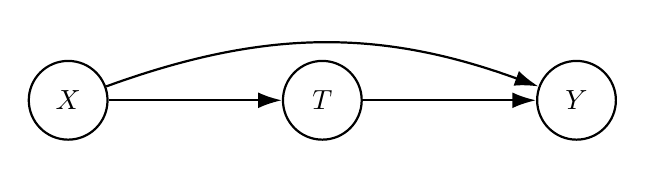
\begin{tikzpicture}[node distance=2.2cm]
        \node[dagnode] (X) {$X$};
        \node[dagnode, right=of X] (T) {$T$};
        \node[dagnode, right=of T] (Y) {$Y$};
        \draw[dagarrow] (X) -- (T);
        \draw[dagarrow] (X) to[out=20,in=160] (Y);
        \draw[dagarrow] (T) -- (Y);
    \end{tikzpicture}
    \caption{Causal structure assumed throughout. The treatment $T$ is continuous and
    possibly multidimensional, the outcome $Y$ is scalar, and the covariates $X$ affect
    both. The only backdoor path $T \leftarrow X \rightarrow Y$ is blocked by
    conditioning on $X$.}
    \label{fig:dag}
\end{figure}

To turn this structure into identification of the potential outcomes
$\{Y(t) : t \in \cT\}$, we impose the standard conditions for continuous treatments
\citep{imbens2000,hirano2004}.

\begin{assumption}[Identification]
\label{as:identification}
Let $t \in \cT$ be the treatment level of interest.
\begin{enumerate}
\item[(i)] \emph{Consistency and no interference.} $Y = Y(T)$, and a unit's potential
outcomes do not depend on the treatment levels of other units.
\item[(ii)] \emph{Weak unconfoundedness.} $Y(t) \perp T \mid X$.
\item[(iii)] \emph{Positivity.} There exists $\gps_{\min} > 0$ such that
$\pf{T \mid X=x}(t) \ge \gps_{\min}$ for every $x$ with $\pf{X}(x) > 0$.
\end{enumerate}
\end{assumption}

Assumption (i) links the potential outcomes to the data, equating the observed $Y$ with
the potential outcome at the treatment received. Assumption (ii) is the distributional
form of the missing common cause of $T$ and $Y$ in Figure~\ref{fig:dag}: given $X$, the
treatment is independent of the potential outcome. Assumption (iii) requires the level $t$
to have positive conditional density at every covariate value; its lower bound
$\gps_{\min}$ will control the correction of Section~\ref{sec:eif}.

Under these assumptions $Y(t)$ is identified. At $X=x$, weak unconfoundedness makes the
conditional density of $Y$ at $T=t$ equal to the density of $Y(t)$, and averaging over the
covariates recovers the interventional density.

\begin{mydef}[Interventional density]
\label{def:target}
For $t \in \cT$ and $y \in \cY$,
\begin{equation}
p_t(y) \;:=\; \pf{Y(t)}(y) \;=\; \pE_X\big[\pf{Y \mid T=t,X}(y)\big]
\;=\; \int_{\cX} \pf{Y \mid T=t,X=x}(y)\,\pf{X}(x) \dd x .
\label{eq:target}
\end{equation}
\end{mydef}

Two features of~\eqref{eq:target} shape the rest of the paper. First, the covariate is
integrated out, whereas $t$ and $y$ are fixed points at which the density is evaluated;
this asymmetry between an averaged and two evaluated arguments is what produces the point
masses in the influence function of Section~\ref{sec:eif}. Second, the only unknown is the
conditional density $\pf{Y \mid T=t,X=x}(y)$ -- the covariate distribution is estimated by
the empirical distribution of $X_1,\dots,X_n$ -- and its conditioning set $(T,X)$ has
dimension $d+p$ while the outcome is scalar; this asymmetry makes standard estimators
inaccurate and dictates the choice of estimator in Section~\ref{sec:setting-mcd}.

The correction of Section~\ref{sec:eif} will also call on the conditional law of the
treatment.

\begin{mydef}[Generalized propensity score]
\label{def:gps}
The conditional density of the treatment given the covariates,
\begin{equation}
\gps(t \mid x) \;:=\; \pf{T \mid X=x}(t),
\label{eq:gps}
\end{equation}
is the generalized propensity score of \citet{imbens2000} and \citet{hirano2004}.
\end{mydef}

For a continuous treatment $\gps(t\mid x)$ is a density in $t \in \R^{d}$, not a
probability, and Assumption~\ref{as:identification}(iii) bounds it below. It plays no role
in identification and enters only through the correction of Section~\ref{sec:eif}; the cost
of estimating it will motivate Section~\ref{sec:mcd-correction}.

\subsection{The conditional density estimator}
\label{sec:setting-mcd}

By~\eqref{eq:target}, estimating $p_t(y)$ comes down to estimating the conditional density
$\pf{Y \mid T=t,X=x}(y)$ and averaging it over the covariates. Any estimator of that
density may be used, and the correction of Section~\ref{sec:eif} does not depend on the
choice; but the choice fixes the accuracy, and the configuration is hostile to classical
estimators. Their rates fall with the dimension of the conditioning argument
\citep{stone1980,Tsybakov2009NonparametricEstimation,bashtannyk2001,hall2004}, here $d+p$,
so with several treatments and confounders this error dominates everything else.

Marginal contrastive discrimination avoids fitting any density on $\cT \times \cX$. It
replaces the conditional density by two objects that are individually easy: the univariate
marginal $\pf{Y}$, and a density ratio obtained by binary classification, which any
supervised learner can solve. On problems of this shape the method is competitive with
state-of-the-art conditional density estimators at lower cost; see \citet{meziani2025mcd}
for the comparisons. We use it with conditioning variable $(T,X)$ and target variable $Y$.
It starts from the elementary factorization
\begin{equation}
\pf{Y \mid T=t,X=x}(y)
\;=\; \pf{Y}(y) \cdot \DensityRatio(t,x,y),
\qquad
\DensityRatio(t,x,y) := \frac{\pf{T,X,Y}(t,x,y)}{\pf{T,X}(t,x)\,\pf{Y}(y)} ,
\label{eq:reformulation}
\end{equation}
valid when $\pf{T,X}(t,x) > 0$ and $\pf{Y}(y) > 0$. The first factor is the univariate
marginal. The second is the density of the joint law relative to the product of its
marginals, and is what the classifier recovers, as follows.

\begin{mydef}[Marginal contrast function, $\MCF(\ratio)$]
\label{def:MCF}
For a mixture ratio $\ratio \in (0,1)$,
\begin{equation}
\contrast(t,x,y)
\;=\; \frac{\ratio\,\pf{T,X,Y}(t,x,y)}
{\ratio\,\pf{T,X,Y}(t,x,y) + (1-\ratio)\,\pf{T,X}(t,x)\,\pf{Y}(y)} .
\label{eq:contrast}
\end{equation}
\end{mydef}

The contrast function is a posterior probability: $\contrast(t,x,y) = \pP[Z=1 \mid W=(t,x,y)]$
in the experiment where a label $Z\in\{0,1\}$ is drawn with $\pP(Z=1)=\ratio$; when $Z=1$
one records an observed vector $W=(T,X,Y)$, and when $Z=0$ one records
$W=(T,X,\widetilde Y)$ with $\widetilde Y \sim \pf{Y}$ independent of $(T,X)$. Estimating
$\contrast$ is thus a supervised classification problem. In practice one builds a
contrastive dataset $\mDwz{N}=\{(W_i,Z_i)\}_{i=1}^{N}$ reproducing this experiment -- the
condition $\MDC(\ratio)$ of \citet{meziani2025mcd} -- by labelling each observed vector
$Z=1$ and adjoining vectors with resampled outcomes labelled $Z=0$.

Since $\contrast$ and $\DensityRatio$ are two encodings of the same information, one
recovers the other, and hence the conditional density.

\begin{mypropo}[Reconstruction identity]
\label{prop:reconstruction}
For all $(t,x,y)$ with $\pf{T,X}(t,x) > 0$ and $\pf{Y}(y) > 0$,
\begin{equation}
\pf{Y \mid T=t,X=x}(y) \;=\; \pf{Y}(y)\,\DensityRatio(t,x,y),
\qquad
\DensityRatio(t,x,y) \;=\; \frac{1-\ratio}{\ratio}\,
\frac{\contrast(t,x,y)}{1-\contrast(t,x,y)} .
\label{eq:reconstruction}
\end{equation}
\end{mypropo}

This is Lemma~1 of \citet{meziani2025mcd} with conditioning variable $(T,X)$, recalled in
Appendix~\ref{app:mcd-reconstruction}. The mixture ratio $\ratio$ is a design parameter:
different values give different contrast functions but the same density ratio, as long as
the value used to build $\mDwz{N}$ is the one used in~\eqref{eq:reconstruction}.

Two features of the construction return in the correction. The negative class is built
from the data by recombination, so the classifier's training law is itself a functional of
$F$; this is what changes the influence function computation in
Section~\ref{sec:mcd-if-classifier}. And because the classifier only compares observed
vectors with recombined ones, it works on the support of the joint law rather than on the
ambient space, which is why the construction stays feasible when $d+p$ is large
\citep{meziani2025mcd}.

\subsection{The plug-in estimator and its first-order bias}
\label{sec:setting-plugin}

Let $\widehat\eta(x) := \pfhat{Y\mid T=t,X=x}(y)$ be any estimator of the conditional
outcome density $\eta(x) := \pf{Y\mid T=t,X=x}(y)$.
Averaging $\widehat\eta$ over the covariates, as~\eqref{eq:target} prescribes, gives the
plug-in estimator
\begin{equation}
\widehat p^{\,\mathrm{pi}}_t(y)
\;=\; \frac{1}{n} \sum_{i=1}^{n} \widehat\eta(X_i).
\label{eq:plugin}
\end{equation}

To analyse its error, suppose $\widehat\eta$ is fitted on a sample independent of
$X_1,\dots,X_n$, and add and subtract the covariate average of the true $\eta$. The error
splits into two parts,
\begin{equation}
\widehat p^{\,\mathrm{pi}}_t(y) - p_t(y)
= \underbrace{\frac1n \sum_{i=1}^n \big( \eta(X_i) - p_t(y) \big)}_{\text{sampling error}}
\;+\; \underbrace{\frac1n \sum_{i=1}^n \big( \widehat\eta(X_i) - \eta(X_i) \big)}_{\text{nuisance error}} ,
\label{eq:plugin-decomp}
\end{equation}
which behave in opposite ways. The sampling error averages the fixed function
$x\mapsto\eta(x)-p_t(y)$ over the covariates, and this function has mean zero, since
$\pE_X[\eta(X)] = p_t(y)$ by~\eqref{eq:target}; the sampling error is therefore centred and
of order $n^{-1/2}$, the usual stochastic fluctuation of a sample mean.

The nuisance error behaves differently, and it is worth seeing why. Because $\widehat\eta$
is fitted on a separate sample, we may treat it as fixed and take expectations over
$X_1,\dots,X_n$ only. Each term $\widehat\eta(X_i)-\eta(X_i)$ then has the same expectation
$\pE_X[\widehat\eta(X)-\eta(X)]$, so
\begin{equation}
\pE\Big[\, \widehat p^{\,\mathrm{pi}}_t(y) - p_t(y) \,\Big|\, \widehat\eta \,\Big]
= \pE_X\big[ \widehat\eta(X) - \eta(X) \big],
\label{eq:plugin-bias}
\end{equation}
the error of the conditional density estimate, averaged over the covariate distribution.
Unlike the sampling error, there is no reason for this quantity to vanish: if $\widehat\eta$
over- or under-estimates $\eta$ on average, so does the plug-in. The nuisance error is thus
not centred but carries a systematic offset, equal to the average error of $\widehat\eta$.
This holds for every conditional density estimator: the offset is a property of the
back-door plug-in, not of any particular $\widehat\eta$.

Term~\eqref{eq:plugin-bias} is what the semiparametric literature calls the first-order
bias of the plug-in, and its name should be read with care, since it is not the bias of an
estimator in the elementary sense. The finite-sample bias $\pE[\widehat\theta]-\theta$ at a
fixed model would vanish as the nuisance became consistent; \eqref{eq:plugin-bias} is a
different object, the leading term of the estimation error expanded in the nuisance error
$\widehat\eta-\eta$, and it is of first order precisely because it is linear in that error.
The same term recurs throughout the literature under names that stress different aspects of
it: an obstruction to efficient estimation with an infinite-dimensional nuisance
\citep{bickel1988,robins2008}, a regularization bias inherited from the smoothing that any
flexible estimator applies \citep{chernozhukov2018}, or the plug-in bias that the one-step
correction is designed to remove \citep{vanderlaan2006tmle,kennedy2022review}. We use the
term first-order bias, meaning by it the object~\eqref{eq:plugin-bias}.

A larger sample does not remove this bias. The nuisance error does shrink as $n$ grows, but
only at the rate of $\|\widehat\eta-\eta\|$, which for a conditional density on a
conditioning set of dimension $d+p$ is slower than $n^{-1/2}$ for any flexible estimator
(Section~\ref{sec:setting-mcd}). On the $\sqrt n$ scale the first-order bias therefore
diverges rather than settling, so $\sqrt n\big(\widehat p^{\,\mathrm{pi}}_t(y)-p_t(y)\big)$
has no centred limit and yields no valid confidence interval. The obstruction is not a
small sample but the sub-parametric rate of conditional density estimation in high
dimension, which no sample size and no choice of estimator overcomes.

This consequence is more damaging for the interventional density than for a mean. The
density is estimated pointwise in $y$, so the first-order bias is not one mislocated number
but a systematic distortion of the whole curve $y\mapsto\widehat p_t(y)$. The quantities
that motivate estimating a density in the first place -- tail probabilities, dispersion,
the probability of exceeding a threshold -- are all functionals of this curve, and each
inherits the distortion. Correcting the first-order bias is thus a prerequisite for the
very inferences the interventional density is meant to support, not a mere refinement.

The correction modifies the estimator so that the nuisance enters only at second order. A
second-order term is quadratic in $\widehat\eta-\eta$, of order $\|\widehat\eta-\eta\|^2$,
and is $o(n^{-1/2})$ as soon as the nuisance converges faster than $n^{-1/4}$ -- a
requirement far weaker than the parametric rate. Achieving this is the one-step correction
of the next section, and it is what makes the influence function necessary.




\section{First-order correction}
\label{sec:eif}

The plug-in estimator~\eqref{eq:plugin} is not $\sqrt{n}$-consistent: its
bias~\eqref{eq:plugin-bias} inherits the slow convergence of the conditional density
estimate and dominates the stochastic error. This section removes that bias. The tool is
the von Mises expansion, which measures how the target responds to a small perturbation of
$F$ and identifies the correction term that cancels the first-order error. We first recall
the expansion, then apply it to $p_t(y)$. The correction we obtain is valid but involves a
new nuisance, the generalized propensity score, which motivates the alternative derivation
of Section~\ref{sec:mcd-correction}.

\subsection{Von Mises expansion}
\label{sec:eif-vm}

View the target as a functional $\psi(F) = p_t(y)$ of the data law. To probe its
sensitivity to the data, perturb $F$ towards a point mass at $w \in \cW$,
\begin{equation}
F_\varepsilon \;=\; (1-\varepsilon)F + \varepsilon\,\delta_w ,
\qquad \varepsilon \in [0,1),
\label{eq:perturbation}
\end{equation}
and differentiate the target along this path.

\begin{mydef}[Influence function]
\label{def:if}
The influence function of $\psi$ at $F$ in the direction $\delta_w$ is
\begin{equation}
\IF(w;\psi,F) \;:=\;
\frac{\partial}{\partial \varepsilon} \psi(F_\varepsilon)\Big|_{\varepsilon=0} .
\label{eq:if-def}
\end{equation}
\end{mydef}

Because $\varepsilon \mapsto \psi(F_\varepsilon)$ is real-valued, this derivative obeys the
ordinary sum, product, quotient and chain rules (Appendix~\ref{app:toolbox}), which is all
we need to compute it below. The influence function has mean zero,
$\pE_F[\IF(W;\psi,F)] = 0$, and controls the first-order response of $\psi$ to a change of
law: for any $F'$,
\begin{equation}
\psi(F') - \psi(F)
\;=\; \pE_{F'}\big[\IF(W;\psi,F)\big] + \Rem_2(F',F),
\label{eq:von-mises}
\end{equation}
with a remainder of second order in $F'-F$. Equation~\eqref{eq:von-mises} is what makes
bias removal possible. Taking $F'$ to be the true law and $F$ the estimated one, the
plug-in error is the first-order term plus a second-order remainder; adding the empirical
average of the estimated influence function to the plug-in cancels that first-order term,
leaving only the remainder. This is the one-step correction
\citep{bickel1993,vandervaart1998} underlying targeted learning \citep{vanderlaan2006tmle}
and debiased machine learning \citep{chernozhukov2018}. It remains to compute
$\IF(w;p_t(y),F)$.

\subsection{The influence function of the interventional density}
\label{sec:eif-classical}

We apply Definition~\ref{def:if} to the target~\eqref{eq:target}. The target is an integral
over $x$ of a ratio of densities in $(t,x,y)$; differentiating it along $F_\varepsilon$
with the calculus of Appendix~\ref{app:toolbox} gives the following.

\begin{mypropo}[Nonparametric correction]
\label{prop:eif}
Under Assumption~\ref{as:identification} and the regularity conditions of
Appendix~\ref{app:classical}, the influence function of $p_t(y)$ at $F$, evaluated at
$w = (t_w,x_w,y_w)$, is
\begin{equation}
\IF\big(w; p_t(y), F\big)
= \frac{\delta_{t_w}(t)}{\gps(t \mid x_w)}
\Big( \delta_{y_w}(y) - \pf{Y \mid T=t,X=x_w}(y) \Big)
+ \pf{Y \mid T=t,X=x_w}(y) - p_t(y),
\label{eq:eif-dirac}
\end{equation}
where $\delta_a$ denotes the Dirac measure at $a$.
\end{mypropo}

The form of~\eqref{eq:eif-dirac} follows the structure of the target noted after
Definition~\ref{def:target}. The covariate is integrated out, so the last two terms are
real-valued and compare the conditional density at the contaminating value $x_w$ with its
average $p_t(y)$. The treatment and outcome are evaluation points, so the first term is
singular: it carries a Dirac in $t$ and in $y$. Crucially, it is weighted by
$1/\gps(t\mid x_w)$, the inverse generalized propensity score of Definition~\ref{def:gps}.
The correction thus depends on $\gps$, an object absent from the target~\eqref{eq:target}.

Two limiting cases place~\eqref{eq:eif-dirac} in the literature. For a discrete treatment
it reduces to the influence function of \citet{kennedy2023density}; for the mean
$\pE[Y(t)]$ it reduces to that of \citet{kennedy2017continuous}. The present target
combines a continuous treatment with a pointwise outcome, and both features appear
together. To our knowledge, this influence function has not been derived before for a
continuous treatment with a pointwise density target; it is contribution~(C1).

The Dirac measures are not estimable, so we regularize them by kernel smoothing with
bandwidths $h_T$ and $h_Y$. Substituting the resulting influence function into the one-step
construction of~\eqref{eq:von-mises} gives the corrected estimator
\begin{equation}
\widehat p^{\,\mathrm{c}}_t(y)
= \frac{1}{n}\sum_{i=1}^{n}
\left[ \frac{K_{h_T}(T_i-t)}{\widehat\gps(t \mid X_i)}
\Big( K_{h_Y}(Y_i-y) - \pfhat{Y \mid T=t,X=X_i}(y) \Big)
+ \pfhat{Y \mid T=t,X=X_i}(y) \right],
\label{eq:est-classical}
\end{equation}
derived in full in Appendix~\ref{app:classical-kernels}. Smoothing enters only through the
two point evaluations; the nuisances $\gps$ and $\pf{Y\mid T,X}$ are unsmoothed and may be
estimated by any method. This estimator corrects the first-order bias of the plug-in, as
the following makes precise.

\begin{mypropo}[Double robustness]
\label{prop:dr-classical}
Under the conditions of Appendix~\ref{app:classical-remainder}, the second-order remainder
of~\eqref{eq:est-classical} factorizes as a product of the errors of $\gps$ and
$\pf{Y\mid T,X}$. Hence $\widehat p^{\,\mathrm{c}}_t(y)$ is $\sqrt{n}$-consistent whenever
each nuisance converges at rate $n^{-1/4}$, and one may converge more slowly if the other
converges faster.
\end{mypropo}

\subsection{The cost of the correction}
\label{sec:eif-cost}

The correction of~\eqref{eq:est-classical} works, but its price is the second nuisance
$\gps$ introduced by~\eqref{eq:eif-dirac}. For a vector treatment, $\gps$ is a conditional
density on $\R^{d}$, and estimating it suffers the same rate degradation that made the
plug-in slow in the first place (Section~\ref{sec:setting-mcd}). The correction has
therefore reintroduced, as a second nuisance, exactly the kind of object the contrastive
construction was chosen to avoid. Double robustness would let one nuisance be slow if the
other were fast, but here $\gps$ and $\pf{Y\mid T,X}$ are both conditional densities in the
treatment coordinate, and both are slow.

The way out uses a property of the influence function itself: it is a functional derivative
of the target and is therefore unique, but the target can be written in several equivalent
forms, and differentiating each yields a different-looking but equal expression for the
same $\IF$. So far we differentiated the target in the form~\eqref{eq:target}, which
produced $\gps$. The contrastive reconstruction~\eqref{eq:reconstruction} gives an
alternative form of the target. Section~\ref{sec:mcd-correction} differentiates that form
instead, and obtains an expression for the same influence function in which $\gps$ no
longer appears and $\pf{Y\mid T,X}$ enters only through its two contrastive factors.

\section{Correction through the contrastive factorization}
\label{sec:mcd-correction}

\subsection{The contrastive form of the correction}
\label{sec:mcd-form}

This subsection establishes the central result of the paper, contribution~(C2): the same
influence function, recomputed from the contrastive factorization, no longer contains the
generalized propensity score.

Substituting the reconstruction identity~\eqref{eq:reconstruction}
into~\eqref{eq:target} factorizes the target as
\begin{equation}
p_t(y) \;=\; \pf{Y}(y)\,m(t,y),
\qquad
m(t,y) \;:=\; \pE_X\big[\DensityRatio(t,X,y)\big] .
\label{eq:factorization}
\end{equation}
Both factors are functionals of $F$, and both are estimated from the same data, so a
perturbation of $F$ moves them jointly. Differentiating~\eqref{eq:factorization} gives
the following.

\begin{mypropo}[Contrastive form]
\label{prop:if-mcd}
Under the conditions of Appendix~\ref{app:mcd}, with $\contrast$ evaluated at $(t,X,y)$
inside the expectations,
\begin{equation}
\begin{aligned}
\IF\big(w;p_t(y),F\big)
&= \pf{Y}(y)\left\{
\DensityRatio(t,x_w,y) - m(t,y)
+ \frac{1-\ratio}{\ratio}\,
\pE_X\!\left[ \frac{\IF\big(w;\contrast,F\big)}{\big(1-\contrast\big)^{2}} \right]
\right\} \\
&\quad + m(t,y)\Big( \delta_{y_w}(y) - \pf{Y}(y) \Big).
\end{aligned}
\label{eq:if-mcd}
\end{equation}
\end{mypropo}

The derivation is in Appendix~\ref{app:mcd-derivation}. The first two terms describe the
variation of the density ratio at the contaminating covariate. The third carries the
influence function of the contrast function itself, and is the subject of
Section~\ref{sec:mcd-if-classifier}. The last term is the correction associated with the
univariate marginal, and is the only place where a point evaluation survives: the outcome
is evaluated at $y$ inside $\pf{Y}(y)$, and the corresponding Dirac measure is
regularized by $K_{h_Y}$ as in Section~\ref{sec:eif-classical}. No Dirac measure appears
in the treatment argument, since the contrast function is evaluated at $(t,X,y)$ through a
model rather than through a point mass of the data.

The generalized propensity score does not appear in~\eqref{eq:if-mcd}. The conditional
outcome density does, since $\pf{Y}(y)\,\DensityRatio(t,x_w,y)$ is that density by
Proposition~\ref{prop:reconstruction}, but only through the two factors
of~\eqref{eq:reformulation}: a univariate density and a contrast function, neither of
which is a conditional density in the treatment coordinate. Since the influence function
is unique, \eqref{eq:if-mcd} must nevertheless agree with~\eqref{eq:eif-dirac}.

\begin{mypropo}[Equivalence]
\label{prop:equivalence}
Suppose $\contrast$ is the contrast function~\eqref{eq:contrast} associated with $F$.
Then~\eqref{eq:if-mcd} reduces to
\begin{equation}
\IF\big(w;p_t(y),F\big)
= \pf{Y \mid T=t,X=x_w}(y) - p_t(y)
+ \pE_X\Big[\IF\big(w;\pf{Y \mid T=t,X}(y),F\big)\Big],
\label{eq:if-collapsed}
\end{equation}
which coincides with~\eqref{eq:eif-dirac}.
\end{mypropo}

Appendix~\ref{app:mcd-equivalence} proves this by direct computation. Two terms produced
by the factorization, one arising from the derivative of the density ratio and one from
the derivative of the marginal, cancel exactly, so that the marginal $\pf{Y}$ leaves no
trace in the reduced expression.

Proposition~\ref{prop:equivalence} also locates the generalized propensity score in the
contrastive form. Unfolding the third term of~\eqref{eq:if-mcd} reproduces the weight
$\delta_{t_w}(t)/\gps(t \mid x_w)$ of~\eqref{eq:eif-dirac}. The propensity score has not
disappeared from the correction; it has been absorbed into the influence function of the
contrast function, and is no longer an object that must be estimated separately.

\subsection{The influence function of the contrast estimate}
\label{sec:mcd-if-classifier}

Evaluating~\eqref{eq:if-mcd} requires $\IF(w;\contrast,F)$, the derivative of the fitted
contrast function with respect to the data-generating law. Influence functions of trained
models have been studied in several literatures. The sandwich formula for penalized
$M$-estimators is classical, and \citet{avella2017} gives a modern treatment.
\citet{kohliang2017} introduced influence functions as a tool for interpreting trained
predictors, and their behaviour in that context was examined by \citet{basu2021} and
\citet{bae2022}. All of these formulas describe the effect of perturbing a fixed training
distribution.

The contrastive construction does not fit this description. The negative class of
$\mDwz{N}$ is generated from the observed data, so the law of the training sample depends
on $F$ through two of its marginals. Perturbing $F$ therefore perturbs the training
distribution as well as the evaluation distribution, and the resulting derivative
contains terms that the classical formula does not.

To make this precise, write the two component laws of the contrastive experiment as
\begin{equation}
P_1(F) := F_{T,X,Y}, \qquad
P_0(F) := F_{T,X} \otimes F_Y ,
\label{eq:laws}
\end{equation}
and let $\pE_{P_\ratio} := \ratio\,\pE_{P_1} + (1-\ratio)\,\pE_{P_0}$ denote expectation
under the mixture prescribed by $\MDC(\ratio)$. The law $P_0(F)$ is a product of two
marginals of $F$, and both factors are affected by a contamination of $F$.

\subsection{The penalized logistic contrast}
\label{sec:mcd-logistic}

We now specialize to a contrast estimate obtained by penalized logistic regression on a
fixed feature map. This is the loss under which \citet{meziani2025mcd} establish the
Bayes optimality of the contrast function, and it has the regularity required for the
derivative above to exist: the training criterion is strictly convex, its minimizer
solves the first-order condition exactly, and its Hessian is invertible with an explicit
lower bound on its spectrum.

Let $\sigma(u) = (1+e^{-u})^{-1}$, let $\phi : \cW \to \R^{\ks}$ be a fixed feature map,
and set $D_\beta(w) = \sigma\big(\beta^\top \phi(w)\big)$. With
$\ell(D,z) = -z\log D - (1-z)\log(1-D)$ the logistic loss, define the penalized risk and
its minimizer
\begin{equation}
\cR_\lambda(\beta;F) := \pE_{P_\ratio}\big[\ell(D_\beta(W),Z)\big]
+ \lambda \|\beta\|_2^2 ,
\qquad
\beta_\lambda(F) := \arg\min_{\beta} \cR_\lambda(\beta;F),
\label{eq:criterion}
\end{equation}
with $\lambda \ge 0$. Write $H_\lambda := \nabla^2_\beta \cR_\lambda(\beta_\lambda;F)$
for the Hessian at the minimizer.

\begin{assumption}[Regularity]
\label{as:smooth}
$\lambda > 0$, the feature map $\phi$ is bounded on $\cW$, and $D_{\beta_\lambda}$ is
bounded away from $0$ and $1$ on the support of $P_\ratio$.
\end{assumption}

Appendix~\ref{app:logistic-grads} shows that under Assumption~\ref{as:smooth} the
criterion~\eqref{eq:criterion} is strictly convex, so $\beta_\lambda(F)$ exists and is
unique, and that every eigenvalue of $H_\lambda$ is at least $2\lambda$. The case
$\lambda = 0$ is admissible provided $\phi$ is not collinear on the support.

\begin{theorem}[Influence function of the contrast estimate]
\label{thm:channels}
Under Assumption~\ref{as:smooth}, with $\beta = \beta_\lambda(F)$ and
$w = (t_w,x_w,y_w)$,
\begin{equation}
\IF\big(w;\beta_\lambda,F\big) \;=\; -\,H_\lambda^{-1}\,\score(w;\beta),
\qquad
\score \;=\; \score_1 + \score_0^{TX} + \score_0^{Y},
\label{eq:master}
\end{equation}
where, with $u_\beta$ and $v_\beta$ the gradients of the loss at labels $1$ and $0$,
\begin{equation}
\begin{aligned}
\score_1 &= \ratio\Big( u_\beta(w) - \pE_{P_1}[u_\beta] \Big), \\
\score_0^{TX} &= (1-\ratio)\Big(
\pE_{\widetilde Y \sim F_Y}\big[ v_\beta(t_w,x_w,\widetilde Y) \big]
- \pE_{P_0}[v_\beta] \Big), \\
\score_0^{Y} &= (1-\ratio)\Big(
\pE_{(T,X) \sim F_{T,X}}\big[ v_\beta(T,X,y_w) \big]
- \pE_{P_0}[v_\beta] \Big).
\end{aligned}
\label{eq:channels}
\end{equation}
\end{theorem}

The three-channel form is contribution~(C3), and it is the key departure from the
classical sandwich formula. The proof is in Appendix~\ref{app:logistic-channels}
and~\ref{app:logistic-ift}. The first channel is the usual score of an $M$-estimator,
computed under the law of the observed data. The other two arise from the contrastive law: since $P_0(F)$ is a product
of two marginals of $F$, contaminating $F$ contaminates each factor separately, and the
derivative of the product contains one term per factor. These two channels are absent
from the formulas of \citet{avella2017} and \citet{kohliang2017}. They also vanish when
the negative class is generated from a distribution fixed by the analyst, as in
noise-contrastive estimation \citep{gutmann2010nce}, in which case~\eqref{eq:master}
reduces to the classical sandwich formula; this is verified in
Appendix~\ref{app:logistic-centering}.

For the logistic model the three channels admit a closed form. Define
\begin{equation}
b_{TX}(t_w,x_w) := \pE_{\widetilde Y \sim \pf{Y}}
\big[ D_\beta \phi (t_w,x_w,\widetilde Y) \big],
\quad
b_Y(y_w) := \pE_{(T,X) \sim \pf{T,X}}
\big[ D_\beta \phi (T,X,y_w) \big],
\quad
b_0 := \pE_{P_0}\big[ D_\beta \phi \big].
\label{eq:b-channels}
\end{equation}

\begin{mypropo}[Closed form]
\label{prop:closed-form}
Under Assumption~\ref{as:smooth},
\begin{equation}
\score(w;\beta)
= \ratio\big( D_\beta(w) - 1 \big)\phi(w)
+ (1-\ratio)\Big( b_{TX}(t_w,x_w) + b_Y(y_w) - b_0 \Big)
+ 2\lambda\beta_\lambda .
\label{eq:S}
\end{equation}
\end{mypropo}

The derivation is in Appendix~\ref{app:logistic-centering}. The three channels contribute
three centring terms, one from the observed law and two identical ones from the
contrastive law. The first-order condition of~\eqref{eq:criterion} eliminates the
unknown expectation under $P_1$, but it contains a single contrastive centring term
whereas the channels produce two, so the term $-(1-\ratio)b_0$ remains. The following
lemma confirms that it must.

\begin{lem}[Zero mean]
\label{lem:zero-mean}
$\pE_{W \sim F}\big[\score(W;\beta_\lambda)\big] = 0$, and hence
$\pE_{W \sim F}\big[\IF(W;\beta_\lambda,F)\big] = 0$.
\end{lem}

The proof, in Appendix~\ref{app:logistic-zero-mean}, uses the fact that when $W \sim F$
the pair $(T,X)$ follows $F_{T,X}$ and the outcome follows $F_Y$, so each contrastive
channel averages to $b_0$. Omitting the term $-(1-\ratio)b_0$ would leave a nonzero mean,
which no influence function can have. Lemma~\ref{lem:zero-mean} also provides a numerical
check on any implementation, discussed in Section~\ref{sec:discussion-diagnostics}.

\subsection{The corrected estimator}
\label{sec:mcd-estimator}

Expression~\eqref{eq:if-mcd} requires $\IF(w;\contrast,F)$ only through an expectation
over the covariates. Since $\IF(w;\beta_\lambda,F)$ does not depend on the covariates, it
factors out of that expectation, and the chain rule reduces the correction term to an
inner product.

\begin{corollary}
\label{cor:collapse}
Let $a_\lambda(t,y) := \pE_X\big[ \DensityRatio(t,X,y)\,\phi(t,X,y) \big]$. Then
\begin{equation}
\frac{1-\ratio}{\ratio}\,
\pE_X\!\left[ \frac{\IF\big(w;\contrast(t,X,y),F\big)}{\big(1-\contrast(t,X,y)\big)^{2}} \right]
\;=\; a_\lambda(t,y)^\top\, \IF\big(w;\beta_\lambda,F\big).
\label{eq:collapse}
\end{equation}
\end{corollary}

Setting $\xi(t,y) := H_\lambda^{-1} a_\lambda(t,y)$ and combining
Proposition~\ref{prop:if-mcd}, Theorem~\ref{thm:channels} and
Corollary~\ref{cor:collapse} gives the estimator
\begin{equation}
\widehat p_t(y)
= \frac{1}{n}\sum_{i=1}^{n} \left\{
\pfhat{Y}(y)\Big[
\widehat{\DensityRatio}(t,X_i,y) - \widehat m(t,y)
- \widehat\xi(t,y)^\top \widehat\score(W_i)
\Big]
+ \widehat m(t,y)\Big( K_{h_Y}(Y_i - y) - \pfhat{Y}(y) \Big)
\right\},
\label{eq:estimator}
\end{equation}
where $\widehat m(t,y) = n^{-1}\sum_{j} \widehat{\DensityRatio}(t,X_j,y)$. The estimator
uses no generalized propensity score, and its only bandwidth is $h_Y$, associated with
the point evaluation of the outcome. No smoothing is performed in the treatment
coordinate.

\subsection{Computation}
\label{sec:mcd-algorithm}

Algorithm~\ref{alg:main} implements~\eqref{eq:estimator}. The Hessian is a single average
over the contrastive dataset and is factorized once. The reparametrization by $\xi(t,y)$
moves the linear solve from the $n$ observations to the evaluation points, which are
typically far fewer, leaving one inner product per observation. The vectors $b_{TX}$ and
$b_Y$ require an average over a marginal for each observation; subsampling this inner
average over $S$ draws reduces the cost to $\cO(nS\ks)$, and the induced Monte Carlo
error is of order $S^{-1/2}$ within a term that is itself averaged over the sample.

Cross-fitting \citep{chernozhukov2018} is used throughout: the contrast function and the
marginal density are fitted on one fold and the correction is evaluated on the other,
with the roles exchanged and the two estimates averaged. This removes the empirical
process conditions that would otherwise be needed, and makes the conditional bias
identity~\eqref{eq:plugin-bias} exact.

\begin{algorithm}[htbp]
\caption{Corrected estimator of $p_t(y)$ with a penalized logistic contrast}
\label{alg:main}
\begin{algorithmic}[1]
\State Split the sample into folds $\mathcal{A}$ and $\mathcal{B}$; exchange the roles and average at the end.
\State On $\mathcal{A}$, build $\mDwz{N}$ satisfying $\MDC(\ratio)$ by labelling each observed vector $Z=1$ and adjoining $\kappa$ vectors with resampled outcomes labelled $Z=0$, so that $\ratio = 1/(1+\kappa)$.
\State Fit $\betahat_\lambda$ by penalized logistic regression on $\mDwz{N}$; set $\contrasthat = \sigma(\betahat_\lambda^\top \phi)$ and $\widehat{\DensityRatio} = \tfrac{1-\ratio}{\ratio}\,\contrasthat/(1-\contrasthat)$.
\State Fit $\pfhat{Y}$ on $\mathcal{A}$ and rescale $\pfhat{Y \mid T,X}$ to integrate to one.
\State Form $\widehat H_\lambda$ as the empirical Hessian on $\mDwz{N}$ and factorize it once; form $\widehat b_0$ as an average over the contrastive part of $\mDwz{N}$.
\For{each evaluation point $(t,y)$}
  \State $\widehat a_\lambda(t,y) \gets n^{-1}\sum_j \widehat{\DensityRatio}(t,X_j,y)\,\phi(t,X_j,y)$;
  \State solve $\widehat H_\lambda\, \widehat\xi(t,y) = \widehat a_\lambda(t,y)$.
\EndFor
\For{each $W_i$ in $\mathcal{B}$}
  \State compute $\widehat b_{TX}(T_i,X_i)$ and $\widehat b_Y(Y_i)$ by subsampling the corresponding marginals;
  \State assemble $\widehat \score(W_i)$ from~\eqref{eq:S}.
\EndFor
\State Return $\widehat p_t(y)$ from~\eqref{eq:estimator}.
\end{algorithmic}
\end{algorithm}

\subsection{Asymptotic distribution}
\label{sec:mcd-asymptotics}

The contrast function is estimated within the parametric family indexed by $\phi$, and
the family need not contain $\contrast$. Let
\begin{equation}
\theta_\lambda(t,y) := \pE_X\big[ \pf{Y}(y)\,\DensityRatio_{\beta_\lambda}(t,X,y) \big],
\qquad
\DensityRatio_{\beta} := \frac{1-\ratio}{\ratio}\,\frac{D_\beta}{1-D_\beta},
\label{eq:pseudo-true}
\end{equation}
be the functional evaluated at the minimizer $\beta_\lambda$ of~\eqref{eq:criterion}. It
equals $p_t(y)$ when the model contains the contrast function. The estimation error
decomposes as
\begin{equation}
\widehat p_t(y) - p_t(y)
= \underbrace{\widehat p_t(y) - \theta_\lambda(t,y)}_{\text{estimation}}
+ \underbrace{\theta_\lambda(t,y) - p_t(y)}_{\text{approximation}} .
\label{eq:decomposition}
\end{equation}

\begin{theorem}[Asymptotic normality]
\label{thm:asymptotics}
Under Assumption~\ref{as:smooth}, cross-fitting, and the moment conditions of
Appendix~\ref{app:asymptotics}, the estimation term of~\eqref{eq:decomposition} satisfies
\begin{equation}
\sqrt{n}\,\big( \widehat p_t(y) - \theta_\lambda(t,y) \big)
\;\longrightarrow\; \mathcal{N}(0,V),
\qquad
V = \pf{Y}(y)^2\, a_\lambda^\top H_\lambda^{-1} \Sigma H_\lambda^{-1} a_\lambda ,
\label{eq:sandwich}
\end{equation}
with $\Sigma = \Var\big(\score(W;\beta_\lambda)\big)$. If in addition
$\|D_{\beta_\lambda} - \contrast\|_{L_2} = o(n^{-1/2})$ and $\ks_n/n \to 0$, the same
statement holds with $\theta_\lambda(t,y)$ replaced by $p_t(y)$.
\end{theorem}

The proof is in Appendix~\ref{app:asymptotics-remainder}. The correction reduces the
estimation term to a second-order quantity in $\betahat - \beta_\lambda$, which is the
sense in which the first-order bias~\eqref{eq:plugin-bias} has been removed. The variance
is available in closed form, so confidence intervals require no resampling. The
approximation term is deterministic and enters linearly, and the additional condition of
Theorem~\ref{thm:asymptotics} requires it to be negligible at the parametric scale; this
is the standard requirement for sieve estimators
\citep{white1982,chen2007,farrell2021}.

\section{Discussion}
\label{sec:discussion}

\subsection{What the correction provides}
\label{sec:discussion-dr}

Estimator~\eqref{eq:est-classical} is doubly robust in the pair
$\big(\gps, \pf{Y \mid T,X}\big)$, and~\eqref{eq:estimator} is not doubly robust. The
reason is structural rather than an artefact of the derivation, and two facts establish
it.

The classical pair consists of the two legs of the identified functional, the treatment
law and the outcome law. The contrastive factorization~\eqref{eq:reformulation} splits
the second leg into a marginal and a density ratio and removes the first leg from the
formula. Splitting one leg in two does not create a pair whose errors multiply, and
Proposition~\ref{prop:equivalence} makes this explicit: the correction associated with
$\pf{Y}$ cancels identically, so the marginal leaves no trace in the influence function
and cannot compensate an error in the contrast function.

Moreover, the two factors are not variationally independent.

\begin{mypropo}[Normalization constraint]
\label{prop:normalization}
For every $y$ with $\pf{Y}(y) > 0$,
\begin{equation}
\pE_{(T,X)}\big[ \DensityRatio(T,X,y) \big] = 1 .
\label{eq:normalization}
\end{equation}
\end{mypropo}

The proof is in Appendix~\ref{app:asymptotics-normalization}. The constraint holds for
every $y$, so the contrast function is restricted by the marginal through a continuum of
identities.

What the correction does provide is the removal of the first-order
bias~\eqref{eq:plugin-bias}, which is present regardless of any pairing of nuisances,
together with the closed-form variance of Theorem~\ref{thm:asymptotics} and insensitivity
to the estimation error of $\beta$ at first order. The condition that replaces double
robustness bears on a single object, the approximation error of the contrast model, and
Section~\ref{sec:discussion-diagnostics} describes how it can be assessed.

\subsection{Diagnostics}
\label{sec:discussion-diagnostics}

Four checks are available and their scopes differ.

The empirical mean of $\widehat\score(W_i)$ should be close to zero by
Lemma~\ref{lem:zero-mean}. This detects implementation errors, in particular an omitted
centring term, but holds whether or not the contrast model is correctly specified.

The empirical mean of $\widehat{\DensityRatio}(T_j,X_j,y)$ should be close to one for
each $y$, by Proposition~\ref{prop:normalization}. This assesses the coherence of the
fitted contrast with the marginal, and is the counterpart of the rescaling step of
\citet{meziani2025mcd}.

Varying the dimension of the feature map and plotting $\widehat p_t(y)$ against $\ks$
indicates whether the approximation error has become negligible. Stabilization supports
the additional condition of Theorem~\ref{thm:asymptotics}; continued drift indicates that
it is not met. In simulations where $\gps$ is available, comparison
with~\eqref{eq:est-classical} provides an empirical check of
Proposition~\ref{prop:equivalence}.

Finally, since the density ratio diverges as the contrast approaches one, the fitted
values $\contrasthat$ should not concentrate near one. Such concentration signals a
region where observed and recombined vectors are nearly separable, which is the
contrastive manifestation of a failure of condition (iii) of
Assumption~\ref{as:identification}.

\subsection{Related work}
\label{sec:discussion-lit}

The estimators of the counterfactual density proposed by \citet{kennedy2023density},
\citet{melnychuk2023flows}, \citet{ham2024logconcave} and \citet{martinez2023stein} all
assume a treatment with finitely many levels, and differ in how the density is
represented. The present work concerns instead the treatment argument, and
Section~\ref{sec:eif-classical} shows that the correction for a discrete treatment is the
limiting case of~\eqref{eq:eif-dirac} in which the kernel degenerates into an indicator.
On the continuous-treatment side, \citet{kennedy2017continuous} and \citet{colangelo2020}
target the mean, which is the case where the outcome is integrated rather than evaluated.

The influence function of the contrast estimate relates to the literature on influence
functions of trained models \citep{avella2017,kohliang2017,basu2021,bae2022}, from which
it differs in that the training distribution is itself a functional of the law of the
data. The channels $\score_0^{TX}$ and $\score_0^{Y}$ of Theorem~\ref{thm:channels} are
the consequence, and they vanish when the negative class is drawn from a fixed
distribution, as in \citet{gutmann2010nce}.

\section{Conclusion}
\label{sec:conclusion}

The interventional density of a scalar outcome under a continuous, multidimensional
treatment is the covariate average of a conditional density whose conditioning set
contains the treatment and all confounders. Marginal contrastive discrimination provides
an estimator of that conditional density adapted to this asymmetry, and the resulting
plug-in estimator of the interventional density carries a first-order bias equal to the
covariate average of the nuisance error.

We derived the influence function of the target. It contains two point evaluations, one
in the treatment and one in the outcome, both regularized by kernel smoothing, and it
involves the generalized propensity score, a conditional density in the treatment
coordinate. Re-expressing the same correction through the contrastive factorization
removes both nuisances from the formula and replaces them by the influence function of
the fitted contrast function, which we computed in closed form for a penalized logistic
model. Because the contrastive sample is generated from the observed data, that influence
function has three score channels rather than one, and the two additional channels do not
cancel.

The resulting estimator is asymptotically normal with a variance available in closed
form, uses no generalized propensity score, and performs no smoothing in the treatment
coordinate. It is not doubly robust, and the condition that replaces double robustness
bears on the approximation error of the contrast model alone.

\bibliographystyle{plainnat}
\bibliography{references}

\clearpage
\appendix

\section*{Appendix}
\addcontentsline{toc}{section}{Appendix}

The appendix is organized as follows. Appendix~\ref{app:toolbox} collects the rules of
the perturbation calculus used throughout. Appendix~\ref{app:classical} derives the
influence function of the interventional density and the remainder of the associated
estimator. Appendix~\ref{app:mcd} derives the contrastive form of the correction and
proves its equivalence with the nonparametric form. Appendix~\ref{app:logistic} treats
the penalized logistic contrast. Appendix~\ref{app:asymptotics} contains the
normalization constraint and the asymptotic analysis.

\section{Perturbation calculus}
\label{app:toolbox}

Throughout this appendix $F_\varepsilon = (1-\varepsilon)F + \varepsilon\,\delta_w$ and
$\IF$ is as in Definition~\ref{def:if}. Each rule below is the corresponding rule of
ordinary calculus applied to the real-valued map
$\varepsilon \mapsto \psi(F_\varepsilon)$.

\begin{lem}[Linearity]
\label{lem:sum}
For functionals $\psi_1,\psi_2$ admitting influence functions at $F$ and constants
$a,b \in \R$,
\[
\IF\big(w; a\psi_1 + b\psi_2, F\big)
= a\,\IF(w;\psi_1,F) + b\,\IF(w;\psi_2,F).
\]
\end{lem}

\begin{proof}
Immediate from the linearity of the derivative of
$\varepsilon \mapsto a\psi_1(F_\varepsilon) + b\psi_2(F_\varepsilon)$ at
$\varepsilon = 0$.
\end{proof}

\begin{lem}[Product]
\label{lem:product}
$\IF\big(w;\psi_1\psi_2,F\big)
= \psi_1(F)\,\IF(w;\psi_2,F) + \psi_2(F)\,\IF(w;\psi_1,F)$.
\end{lem}

\begin{proof}
Set $\varphi(\varepsilon) = \psi_1(F_\varepsilon)$ and
$\chi(\varepsilon) = \psi_2(F_\varepsilon)$. The ordinary product rule gives
$\varphi(0)\chi'(0) + \chi(0)\varphi'(0)$, and the values at $\varepsilon = 0$ are
$\varphi(0) = \psi_1(F)$, $\chi(0) = \psi_2(F)$, $\varphi'(0) = \IF(w;\psi_1,F)$ and
$\chi'(0) = \IF(w;\psi_2,F)$.
\end{proof}

\begin{lem}[Quotient]
\label{lem:quotient}
If $\psi_2(F) \neq 0$,
\[
\IF\!\left(w;\frac{\psi_1}{\psi_2},F\right)
= \frac{\IF(w;\psi_1,F)}{\psi_2(F)}
- \frac{\psi_1(F)}{\psi_2(F)^2}\,\IF(w;\psi_2,F).
\]
\end{lem}

\begin{proof}
With $\varphi,\chi$ as above and $\chi(0) \neq 0$, the ordinary quotient rule gives
$\{\varphi'(0)\chi(0) - \varphi(0)\chi'(0)\}/\chi(0)^2$.
\end{proof}

\begin{lem}[Chain rule]
\label{lem:chain}
For $h : \R \to \R$ differentiable,
$\IF\big(w;h \circ \psi,F\big) = h'\big(\psi(F)\big)\,\IF(w;\psi,F)$.
\end{lem}

\begin{proof}
With $\chi(\varepsilon) = \psi(F_\varepsilon)$, the ordinary chain rule gives
$h'(\chi(0))\chi'(0)$.
\end{proof}

\begin{lem}[Odds transformation]
\label{lem:odds}
Let $\psi$ take values in $(0,1)$ and $h(u) = u/(1-u)$. Then
\[
\IF\big(w;h(\psi),F\big) = \frac{\IF(w;\psi,F)}{\big(1-\psi(F)\big)^2} .
\]
In particular, since $\DensityRatio = \frac{1-\ratio}{\ratio} h(\contrast)$ with
$\ratio$ constant,
\begin{equation}
\IF\big(w;\DensityRatio,F\big)
= \frac{1-\ratio}{\ratio}\,
\frac{\IF\big(w;\contrast,F\big)}{\big(1-\contrast\big)^{2}} .
\label{eq:app-if-R}
\end{equation}
\end{lem}

\begin{proof}
Apply Lemma~\ref{lem:quotient} with $\psi_1 = \psi$ and $\psi_2 = 1-\psi$, and use
$\IF(w;1-\psi,F) = -\IF(w;\psi,F)$ from Lemma~\ref{lem:sum}:
\[
\frac{\IF(w;\psi,F)}{1-\psi(F)}
+ \frac{\psi(F)}{(1-\psi(F))^2}\,\IF(w;\psi,F)
= \IF(w;\psi,F)\,\frac{(1-\psi(F)) + \psi(F)}{(1-\psi(F))^2} . \qedhere
\]
\end{proof}

\begin{lem}[Expectation of a law-dependent integrand]
\label{lem:if-expectation}
Let $h(\cdot\,;F)$ depend on $F$ both through the law of the integration variable and
through its functional form. Then
\begin{equation}
\IF\big(w; \pE_F[h(W;F)], F\big)
= h(w;F) - \pE_F\big[h(W;F)\big]
+ \pE_F\big[ \IF(w;h(\cdot\,;F),F) \big].
\label{eq:app-if-expectation}
\end{equation}
\end{lem}

\begin{proof}
By the definition of $F_\varepsilon$,
\[
\pE_{F_\varepsilon}\big[h(W;F_\varepsilon)\big]
= (1-\varepsilon)\,\pE_F\big[h(W;F_\varepsilon)\big]
+ \varepsilon\,h(w;F_\varepsilon).
\]
Differentiating at $\varepsilon = 0$, the factor $(1-\varepsilon)$ contributes
$-\pE_F[h(W;F)]$ and the integrand contributes
$\pE_F[\partial_\varepsilon h(W;F_\varepsilon)|_{0}]$, while the second summand
contributes $h(w;F)$, its own derivative being multiplied by $\varepsilon = 0$.
\end{proof}

The third term of~\eqref{eq:app-if-expectation} accounts for the dependence of the
integrand on the law and is required whenever the integrand is itself estimated.

\section{The nonparametric correction}
\label{app:classical}

\subsection{Regularity conditions}
\label{app:classical-regularity}

Proposition~\ref{prop:eif} is stated under Assumption~\ref{as:identification} together
with the following conditions, which are those of \citet{kennedy2017continuous} and
\citet{kennedy2023density} adapted to the present target. The joint density
$\pf{T,X,Y}$ is bounded and twice continuously differentiable in $(t,y)$ in a
neighbourhood of the evaluation point; the map $y \mapsto \pf{Y}(y)$ is twice
continuously differentiable at $y$; and the kernels $K_T,K_Y$ are symmetric, of second
order, with compact support. The bandwidths satisfy $h_T,h_Y \to 0$,
$n h_T^{d} h_Y \to \infty$, and the undersmoothing conditions
$\sqrt{n h_T^d h_Y}\,(h_T^2 + h_Y^2) \to 0$.

\subsection{Derivation of the influence function}
\label{app:classical-derivative}

Write $f_\varepsilon$ for the density of $F_\varepsilon$ and express the target as
\[
p_t(y)(F_\varepsilon)
= \int_{\cX} \frac{f_\varepsilon(t,x,y)\,f_\varepsilon(x)}{f_\varepsilon(t,x)} \dd x .
\]
The map $\varepsilon \mapsto f_\varepsilon$ is affine, so each density derivative is the
difference between a point mass and the density:
\begin{equation}
\begin{aligned}
\partial_\varepsilon f_\varepsilon(t,x,y)\big|_{0} &= \Delta(t,x,y) - \pf{T,X,Y}(t,x,y),\\
\partial_\varepsilon f_\varepsilon(x)\big|_{0} &= \Delta(x) - \pf{X}(x),\\
\partial_\varepsilon f_\varepsilon(t,x)\big|_{0} &= \Delta(t,x) - \pf{T,X}(t,x),
\end{aligned}
\label{eq:app-density-derivs}
\end{equation}
where $\Delta(t,x,y) := \delta_{t_w}(t)\,\delta_{x_w}(x)\,\delta_{y_w}(y)$ and similarly
for the marginals.

Write the integrand as $AB/C$ with $A = f_\varepsilon(t,x,y)$, $B = f_\varepsilon(x)$ and
$C = f_\varepsilon(t,x)$. Ordinary calculus gives
\[
\partial_\varepsilon\!\left( \frac{AB}{C} \right)
= \frac{\dot A B}{C} + \frac{A \dot B}{C} - \frac{AB\dot C}{C^2},
\]
and substituting~\eqref{eq:app-density-derivs} at $\varepsilon = 0$, then factoring
$\pf{T,X,Y}(t,x,y)\pf{X}(x)/\pf{T,X}(t,x)$ out of the bracket,
\begin{equation}
\partial_\varepsilon\, p_t(y)(F_\varepsilon)\big|_{0}
= \int_{\cX} \frac{\pf{T,X,Y}(t,x,y)\,\pf{X}(x)}{\pf{T,X}(t,x)}
\left[
\frac{\Delta(t,x,y)}{\pf{T,X,Y}(t,x,y)}
+ \frac{\Delta(x)}{\pf{X}(x)}
- \frac{\Delta(t,x)}{\pf{T,X}(t,x)}
- 1
\right] \dd x ,
\label{eq:app-deriv-general}
\end{equation}
the constant $-1$ collecting the three terms $-1-1+1$. We treat the four contributions in
turn.

The term in $\Delta(x)$ involves only the point mass in the integration variable, and
\[
\int_{\cX} \frac{\pf{T,X,Y}(t,x,y)}{\pf{T,X}(t,x)}\,\delta_{x_w}(x)\dd x
= \pf{Y \mid T=t,X=x_w}(y),
\]
the test function being continuous by Appendix~\ref{app:classical-regularity}.

The term in $\Delta(t,x,y)$ carries point masses in $t$ and $y$, which are not
integration variables. Only $\delta_{x_w}(x)$ is integrated, and using
$\gps(t \mid x) = \pf{T,X}(t,x)/\pf{X}(x)$,
\[
\int_{\cX} \frac{\pf{X}(x)}{\pf{T,X}(t,x)}\,
\delta_{t_w}(t)\delta_{x_w}(x)\delta_{y_w}(y)\dd x
= \frac{\delta_{t_w}(t)\,\delta_{y_w}(y)}{\gps(t \mid x_w)} .
\]

The term in $\Delta(t,x)$ carries a point mass in $t$ only, and
\[
-\int_{\cX} \frac{\pf{T,X,Y}(t,x,y)\,\pf{X}(x)}{\pf{T,X}(t,x)^2}\,
\delta_{t_w}(t)\delta_{x_w}(x)\dd x
= -\,\frac{\delta_{t_w}(t)\,\pf{Y \mid T=t,X=x_w}(y)}{\gps(t \mid x_w)} .
\]

The constant term integrates to $-p_t(y)$.

Collecting the four contributions and factoring $\delta_{t_w}(t)$ out of the second and
third gives~\eqref{eq:eif-dirac}. \hfill$\square$

\subsection{Regularization of the point evaluations}
\label{app:classical-kernels}

Expression~\eqref{eq:eif-dirac} is exact but not computable, since it contains Dirac
measures in $t$ and $y$. We regularize each by a kernel. Let $K_T : \R^{d} \to \R_+$ and
$K_Y : \R \to \R_+$ be symmetric second-order kernels integrating to one, and for
bandwidths $h_T, h_Y > 0$ set
\begin{equation}
K_{h_T}(u) = h_T^{-d} K_T(u/h_T), \qquad
K_{h_Y}(v) = h_Y^{-1} K_Y(v/h_Y).
\label{eq:kernels}
\end{equation}
Substituting $\delta_{t_w}(t) \rightsquigarrow K_{h_T}(t_w - t)$ and
$\delta_{y_w}(y) \rightsquigarrow K_{h_Y}(y_w - y)$ in~\eqref{eq:eif-dirac}, and leaving
the nuisances unchanged, gives
\begin{equation}
\IF_{h}\big(w;p_t(y),F\big)
= \frac{K_{h_T}(t_w-t)}{\gps(t \mid x_w)}
\Big( K_{h_Y}(y_w-y) - \pf{Y \mid T=t,X=x_w}(y) \Big)
+ \pf{Y \mid T=t,X=x_w}(y) - p_t(y),
\label{eq:app-if-smoothed}
\end{equation}
whose empirical average added to the plug-in estimator yields~\eqref{eq:est-classical}.
Under Appendix~\ref{app:classical-regularity}, a second-order Taylor expansion of the
smoothed functional around $(t,y)$ shows that
$\pE\big[\IF_h(W;p_t(y),F)\big] = \cO(h_T^2 + h_Y^2)$, so the substitution introduces a
deterministic bias of that order, negligible under the stated undersmoothing conditions.

Two special cases recover known results. If $T$ takes finitely many values, the point
mass $\delta_{t_w}(t)$ is the indicator $\Indi(t_w = t)$, no smoothing is required in the
treatment argument, and $\gps(t \mid x)$ is the propensity score; \eqref{eq:app-if-smoothed}
then reduces to the influence function of \citet{kennedy2023density}. If the target is
$\pE[Y(t)]$, the outcome is integrated rather than evaluated, the derivation carries an
extra factor $y$ and an extra integral in $y$, the point mass $\delta_{y_w}(y)$ is
replaced by $y_w$, and~\eqref{eq:app-if-smoothed} reduces to the influence function of
\citet{kennedy2017continuous}.

\subsection{Second-order remainder}
\label{app:classical-remainder}

Let $\widehat\gps$ and $\pfhat{Y \mid T,X}$ be nuisance estimates fitted on an
independent fold. Writing $\eta(x) := \pf{Y \mid T=t,X=x}(y)$ and
$\widehat\eta(x) := \pfhat{Y \mid T=t,X=x}(y)$, and taking expectations
in~\eqref{eq:est-classical} conditionally on the fitting fold, the terms linear in the
nuisance errors cancel and there remains
\begin{equation}
\Rem_2
= \pE\!\left[
\left( \frac{K_{h_T}(T-t)}{\widehat\gps(t \mid X)}
- \frac{K_{h_T}(T-t)}{\gps(t \mid X)} \right)
\Big( \eta(X) - \widehat\eta(X) \Big)
\right].
\label{eq:app-remainder}
\end{equation}
By the Cauchy-Schwarz inequality and the lower bound $\gps_{\min}$ of
Assumption~\ref{as:identification}(iii),
\[
|\Rem_2| \;\lesssim\; \big\| \widehat\gps - \gps \big\|_{L_2}\,
\big\| \widehat\eta - \eta \big\|_{L_2} ,
\]
which is the double robustness property invoked in Section~\ref{sec:eif-classical}.

\section{The contrastive correction}
\label{app:mcd}

\subsection{Proof of Proposition~\ref{prop:reconstruction}}
\label{app:mcd-reconstruction}

From Definition~\ref{def:MCF}, the odds of the contrast function are
\[
\frac{\contrast}{1-\contrast}
= \frac{\ratio\,\pf{T,X,Y}(t,x,y)}{(1-\ratio)\,\pf{T,X}(t,x)\,\pf{Y}(y)}
= \frac{\ratio}{1-\ratio}\,
\frac{\pf{Y \mid T=t,X=x}(y)}{\pf{Y}(y)} ,
\]
using $\pf{T,X,Y}(t,x,y) = \pf{T,X}(t,x)\,\pf{Y \mid T=t,X=x}(y)$. Multiplying by
$(1-\ratio)/\ratio$ gives
$\DensityRatio = \pf{Y \mid T=t,X=x}(y)/\pf{Y}(y)$, which is~\eqref{eq:reconstruction}.
\hfill$\square$

\subsection{Proof of Proposition~\ref{prop:if-mcd}}
\label{app:mcd-derivation}

Apply Lemma~\ref{lem:product} to the factorization $p_t(y) = \pf{Y}(y)\,m(t,y)$
of~\eqref{eq:factorization}:
\begin{equation}
\IF\big(w;p_t(y),F\big)
= \pf{Y}(y)\,\IF\big(w;m(t,y),F\big)
+ m(t,y)\,\IF\big(w;\pf{Y}(y),F\big).
\label{eq:app-product}
\end{equation}

For the second factor, $\pf{Y}(y)$ depends on $F$ only through the marginal law of the
outcome, evaluated at the fixed point $y$. The computation of
Appendix~\ref{app:classical-derivative}, applied to a univariate marginal, gives
\begin{equation}
\IF\big(w;\pf{Y}(y),F\big) = \delta_{y_w}(y) - \pf{Y}(y),
\label{eq:app-if-fY}
\end{equation}
regularized as in Appendix~\ref{app:classical-kernels} by
$\delta_{y_w}(y) \rightsquigarrow K_{h_Y}(y_w - y)$.

For the first factor, apply Lemma~\ref{lem:if-expectation} to
$m(t,y) = \pE_X[\DensityRatio(t,X,y)]$ with integrand $h(X;F) = \DensityRatio(t,X,y;F)$:
\begin{equation}
\IF\big(w;m(t,y),F\big)
= \DensityRatio(t,x_w,y) - m(t,y)
+ \pE_X\big[ \IF(w;\DensityRatio(t,X,y),F) \big].
\label{eq:app-if-m}
\end{equation}
The third term is present because the density ratio is itself a functional of $F$ through
the contrast function. Substituting~\eqref{eq:app-if-R} of Lemma~\ref{lem:odds}
into~\eqref{eq:app-if-m}, then~\eqref{eq:app-if-m} and~\eqref{eq:app-if-fY}
into~\eqref{eq:app-product}, gives~\eqref{eq:if-mcd}. \hfill$\square$

\subsection{Proof of Proposition~\ref{prop:equivalence}}
\label{app:mcd-equivalence}

Write $\eta(x) := \pf{Y \mid T=t,X=x}(y)$. Assume $\contrast$ is the contrast function
associated with $F$, so that $\DensityRatio(t,x,y) = \eta(x)/\pf{Y}(y)$ by
Proposition~\ref{prop:reconstruction}. Lemma~\ref{lem:quotient} gives
\begin{equation}
\IF\big(w;\DensityRatio(t,x,y),F\big)
= \frac{\IF\big(w;\eta(x),F\big)}{\pf{Y}(y)}
- \frac{\eta(x)}{\pf{Y}(y)^2}\,\IF\big(w;\pf{Y}(y),F\big).
\label{eq:app-if-R-true}
\end{equation}
Taking $\pE_X$ in~\eqref{eq:app-if-R-true} and using $\pE_X[\eta(X)] = p_t(y)$,
\begin{equation}
\pE_X\big[ \IF(w;\DensityRatio(t,X,y),F) \big]
= \frac{\pE_X\big[ \IF(w;\eta(X),F) \big]}{\pf{Y}(y)}
- \frac{p_t(y)}{\pf{Y}(y)^2}\,\IF\big(w;\pf{Y}(y),F\big).
\label{eq:app-Ex}
\end{equation}
The remaining terms of~\eqref{eq:app-if-m} are rewritten with the same identity, namely
$\DensityRatio(t,x_w,y) = \eta(x_w)/\pf{Y}(y)$ and
$m(t,y) = p_t(y)/\pf{Y}(y)$. Substituting these and~\eqref{eq:app-Ex}
into~\eqref{eq:app-if-m} and multiplying by $\pf{Y}(y)$ yields
\[
\pf{Y}(y)\,\IF\big(w;m(t,y),F\big)
= \eta(x_w) - p_t(y) + \pE_X\big[ \IF(w;\eta(X),F) \big]
- \frac{p_t(y)}{\pf{Y}(y)}\,\IF\big(w;\pf{Y}(y),F\big).
\]
The second summand of~\eqref{eq:app-product} equals
$m(t,y)\,\IF(w;\pf{Y}(y),F) = \frac{p_t(y)}{\pf{Y}(y)}\,\IF(w;\pf{Y}(y),F)$ and cancels
the last term of the display, leaving~\eqref{eq:if-collapsed}.

To identify~\eqref{eq:if-collapsed} with~\eqref{eq:eif-dirac}, apply
Lemma~\ref{lem:if-expectation} directly to $p_t(y) = \pE_X[\eta(X)]$:
\[
\IF\big(w;p_t(y),F\big)
= \eta(x_w) - \pE_X[\eta(X)] + \pE_X\big[ \IF(w;\eta(X),F) \big],
\]
which coincides with~\eqref{eq:if-collapsed} term by term. Differentiating
$\eta(x) = \pf{T,X,Y}(t,x,y)/\pf{T,X}(t,x)$ by Lemma~\ref{lem:quotient} and integrating
over $x$ reproduces the first term of~\eqref{eq:eif-dirac}, as in
Appendix~\ref{app:classical-derivative}. \hfill$\square$

The cancellation is exact and not an approximation: the terms introduced by the
factorization sum to zero, and neither $\pf{Y}$ nor $\contrast$ appears individually in
the reduced expression.

\section{The penalized logistic contrast}
\label{app:logistic}

Throughout, $\beta = \beta_\lambda(F)$, $D := D_\beta$, $\phi := \phi(t,x,y)$, and all
expectations are taken at $F$.

\subsection{Gradients, Hessian and convexity}
\label{app:logistic-grads}

Differentiating the logistic loss in its first argument,
\begin{equation}
\frac{\partial \ell}{\partial D}(D,z)
= -\frac{z}{D} + \frac{1-z}{1-D}
= \frac{D-z}{D(1-D)} .
\label{eq:app-dl}
\end{equation}
Differentiating the model in $\beta$, with $\sigma' = \sigma(1-\sigma)$,
\begin{equation}
\nabla_\beta D_\beta = D(1-D)\,\phi .
\label{eq:app-grad-D}
\end{equation}
Composing the two, the factor $D(1-D)$ cancels and
\begin{equation}
\nabla_\beta \ell(D_\beta,z) = (D-z)\,\phi ,
\qquad\text{so}\qquad
u_\beta = (D-1)\phi, \quad v_\beta = D\phi .
\label{eq:app-uv}
\end{equation}
Differentiating once more and using~\eqref{eq:app-grad-D},
$\nabla_\beta u_\beta = \nabla_\beta v_\beta = D(1-D)\phi\phi^\top$, so both labels
contribute the same second derivative and
\begin{equation}
H_\lambda
= \pE_{P_\ratio}\big[ D(1-D)\,\phi\phi^\top \big] + 2\lambda I_{\ks} .
\label{eq:app-hessian}
\end{equation}
For any $s \in \R^{\ks}$,
\[
s^\top H_\lambda s
= \pE_{P_\ratio}\big[ D(1-D)(s^\top\phi)^2 \big] + 2\lambda\|s\|^2
\;\ge\; 2\lambda\|s\|^2 ,
\]
since $D(1-D) > 0$. Hence $H_\lambda$ is positive definite with all eigenvalues at least
$2\lambda$, the criterion~\eqref{eq:criterion} is strictly convex, and $\beta_\lambda(F)$
exists, is unique and is interior. When $\lambda = 0$ the same computation gives positive
definiteness provided $\pE_{P_\ratio}[(s^\top\phi)^2] > 0$ for every $s \neq 0$.

The first-order condition $\nabla_\beta \cR_\lambda = 0$ reads
\begin{equation}
G_\lambda(\beta;F)
:= \ratio\,\pE_{P_1}[u_\beta] + (1-\ratio)\,\pE_{P_0}[v_\beta] + 2\lambda\beta = 0 .
\label{eq:app-foc}
\end{equation}

\subsection{Perturbation of the two component laws}
\label{app:logistic-channels}

The observed law satisfies $P_1(F_\varepsilon) = F_\varepsilon$, and
$\pE_{F_\varepsilon}[u] = (1-\varepsilon)\pE_F[u] + \varepsilon\,u(w)$ is affine in
$\varepsilon$, so
\begin{equation}
\partial_\varepsilon\, \pE_{P_1(F_\varepsilon)}[u]\big|_{0}
= u(w) - \pE_{P_1}[u].
\label{eq:app-channel1}
\end{equation}

The contrastive law is the product
$P_0(F_\varepsilon) = F_{T,X,\varepsilon} \otimes F_{Y,\varepsilon}$, whose factors are
the marginals of $F_\varepsilon$:
\[
F_{T,X,\varepsilon} = (1-\varepsilon)F_{T,X} + \varepsilon\,\delta_{(t_w,x_w)},
\qquad
F_{Y,\varepsilon} = (1-\varepsilon)F_Y + \varepsilon\,\delta_{y_w} .
\]
Expanding the double integral gives four terms, according to which factors carry the
contamination:
\begin{equation}
\begin{aligned}
\pE_{P_0(F_\varepsilon)}[v]
&= (1-\varepsilon)^2\,\pE_{P_0}[v]
+ (1-\varepsilon)\varepsilon\,\pE_{F_{T,X}}\big[ v(T,X,y_w) \big] \\
&\quad + \varepsilon(1-\varepsilon)\,\pE_{F_Y}\big[ v(t_w,x_w,\widetilde Y) \big]
+ \varepsilon^2\, v(t_w,x_w,y_w).
\end{aligned}
\label{eq:app-p0-expanded}
\end{equation}
Differentiating at $\varepsilon = 0$, the quadratic term vanishes, the factor
$(1-\varepsilon)^2$ contributes $-2$, and each cross term contributes $+1$, so
\begin{equation}
\partial_\varepsilon\, \pE_{P_0(F_\varepsilon)}[v]\big|_{0}
= \pE_{F_Y}\big[ v(t_w,x_w,\widetilde Y) \big]
+ \pE_{F_{T,X}}\big[ v(T,X,y_w) \big]
- 2\,\pE_{P_0}[v].
\label{eq:app-channel0}
\end{equation}
The coefficient $-2$ is what splits the contrastive derivative into two channels, one for
each factor of the product measure. Equivalently, Lemma~\ref{lem:product} applied to the
bilinear map $(\mu,\nu) \mapsto \iint v \dd\mu \dd\nu$ gives the first bracket by
differentiating $F_{T,X,\varepsilon}$ at fixed $F_Y$ and the second by differentiating
$F_{Y,\varepsilon}$ at fixed $F_{T,X}$. The mixture ratio $\ratio$ is a design constant
and contributes no derivative.

\subsection{Proof of Theorem~\ref{thm:channels}}
\label{app:logistic-ift}

By definition $\beta_\lambda(F_\varepsilon)$ solves
$G_\lambda\big(\beta_\lambda(F_\varepsilon);F_\varepsilon\big) = 0$ identically in
$\varepsilon$. The left-hand side depends on $\varepsilon$ through the parameter and
through the law, so differentiating at $\varepsilon = 0$,
\begin{equation}
\underbrace{\nabla_\beta G_\lambda}_{=\,H_\lambda}\,
\underbrace{\partial_\varepsilon \beta_\lambda(F_\varepsilon)\big|_{0}}_{=\,\IF(w;\beta_\lambda,F)}
+ \underbrace{\partial_\varepsilon G_\lambda(\beta;F_\varepsilon)\big|_{0}}_{=:\,\score(w;\beta)}
= 0 .
\label{eq:app-ift}
\end{equation}
Since $H_\lambda$ is invertible by Appendix~\ref{app:logistic-grads}, this gives
$\IF(w;\beta_\lambda,F) = -H_\lambda^{-1}\score(w;\beta)$. Applying
\eqref{eq:app-channel1} with $u = u_\beta$ and~\eqref{eq:app-channel0} with
$v = v_\beta$ to
$G_\lambda(\beta;F_\varepsilon) = \ratio\,\pE_{P_1(F_\varepsilon)}[u_\beta]
+ (1-\ratio)\,\pE_{P_0(F_\varepsilon)}[v_\beta] + 2\lambda\beta$,
and noting that the penalty does not depend on $F$, gives the three channels
of~\eqref{eq:channels}. \hfill$\square$

\subsection{Proof of Proposition~\ref{prop:closed-form}}
\label{app:logistic-centering}

By~\eqref{eq:app-uv}, the centring terms of~\eqref{eq:channels} all equal
$\pE_{P_0}[v_\beta] = \pE_{P_0}[D\phi] = b_0$, and the contaminated contrastive terms are
$b_{TX}(t_w,x_w)$ and $b_Y(y_w)$ of~\eqref{eq:b-channels}. Summing the three channels,
\begin{equation}
\score(w;\beta)
= \ratio\,u_\beta(w) + (1-\ratio)\big( b_{TX}(t_w,x_w) + b_Y(y_w) \big)
- \Big( \ratio\,\pE_{P_1}[u_\beta] + 2(1-\ratio)\,b_0 \Big).
\label{eq:app-S-raw}
\end{equation}
The bracket contains the unknown $\pE_{P_1}[u_\beta]$, which the first-order
condition~\eqref{eq:app-foc} determines as
$\ratio\,\pE_{P_1}[u_\beta] = -2\lambda\beta_\lambda - (1-\ratio)b_0$. Substituting,
\begin{equation}
-\Big( \ratio\,\pE_{P_1}[u_\beta] + 2(1-\ratio)b_0 \Big)
= 2\lambda\beta_\lambda + (1-\ratio)b_0 - 2(1-\ratio)b_0
= 2\lambda\beta_\lambda - (1-\ratio)b_0 .
\label{eq:app-resolve}
\end{equation}
The residual $-(1-\ratio)b_0$ arises because the first-order condition contains one
contrastive centring term whereas the three channels produce two. Combining
\eqref{eq:app-S-raw}, \eqref{eq:app-resolve} and $u_\beta = (D-1)\phi$
gives~\eqref{eq:S}. \hfill$\square$

Two limiting cases are worth recording. Setting $\lambda = 0$ removes the last term of
\eqref{eq:S}. Setting in addition the two contrastive channels to zero, which is the
situation of a negative class drawn from a distribution fixed by the analyst, leaves
$\score(w;\beta) = \ratio\big(D_\beta(w)-1\big)\phi(w)$, and~\eqref{eq:master} becomes
$-H_0^{-1}\big(D_\beta(w) - z_w\big)\phi(w)$, the classical influence function of
logistic regression.

\subsection{Proof of Lemma~\ref{lem:zero-mean}}
\label{app:logistic-zero-mean}

Take the expectation of~\eqref{eq:S} over $W \sim F$. Since $W = (T,X,Y)$ is drawn from
$F$, its first two components follow $F_{T,X}$ and its last component follows $F_Y$.

The first term is an expectation under $P_1 = F_{T,X,Y}$, so by~\eqref{eq:app-uv} it
equals $\ratio\,\pE_{P_1}[u_\beta]$.

The vector $b_{TX}(T,X) = \pE_{\widetilde Y \sim F_Y}[v_\beta(T,X,\widetilde Y)]$ is a
function of $(T,X)$ alone. Averaging over $(T,X) \sim F_{T,X}$ and using Fubini together
with the product structure of $P_0$,
\[
\pE\big[ b_{TX}(T,X) \big]
= \pE_{(T,X) \sim F_{T,X}} \pE_{\widetilde Y \sim F_Y}\big[ v_\beta(T,X,\widetilde Y) \big]
= \pE_{P_0}[v_\beta] = b_0 .
\]
Symmetrically, $b_Y(Y) = \pE_{(T,X) \sim F_{T,X}}[v_\beta(T,X,Y)]$ is a function of $Y$
alone and averages to $b_0$.

The vectors $b_0$ and $2\lambda\beta_\lambda$ are constants. Summing,
\[
\pE\big[ \score(W;\beta) \big]
= \ratio\,\pE_{P_1}[u_\beta] + (1-\ratio)\big( b_0 + b_0 - b_0 \big) + 2\lambda\beta_\lambda
= G_\lambda(\beta_\lambda;F) = 0
\]
by~\eqref{eq:app-foc}. Since $H_\lambda$ does not depend on $w$, the second statement
follows from~\eqref{eq:master}. \hfill$\square$

Had the term $-(1-\ratio)b_0$ been omitted from~\eqref{eq:S}, the contrastive
contributions would have summed to $2b_0$ instead of $b_0$ and the total would have been
$(1-\ratio)b_0 \neq 0$, which is impossible for an influence function.

\subsection{Proof of Corollary~\ref{cor:collapse}}
\label{app:logistic-collapse}

By Lemma~\ref{lem:chain} applied to $\beta \mapsto D_\beta(t,x,y)$ at fixed $(t,x,y)$,
together with~\eqref{eq:app-grad-D},
\[
\IF\big(w;\contrast(t,x,y),F\big)
= D(1-D)\,\phi(t,x,y)^\top\,\IF\big(w;\beta_\lambda,F\big).
\]
Dividing by $(1-D)^2$, multiplying by $(1-\ratio)/\ratio$ and taking the expectation over
the covariates, the vector $\IF(w;\beta_\lambda,F)$ does not depend on $X$ and factors
out. The scalar weight simplifies as
\[
\frac{1-\ratio}{\ratio}\,\frac{D(1-D)}{(1-D)^2}
= \frac{1-\ratio}{\ratio}\,\frac{D}{1-D}
= \DensityRatio ,
\]
which gives $a_\lambda(t,y) = \pE_X[\DensityRatio(t,X,y)\phi(t,X,y)]$
and~\eqref{eq:collapse}. \hfill$\square$

Consequently, with $\xi(t,y) = H_\lambda^{-1}a_\lambda(t,y)$ and by the symmetry of
$H_\lambda$,
\[
a_\lambda(t,y)^\top \IF\big(w;\beta_\lambda,F\big)
= -\,\big( H_\lambda^{-1}a_\lambda(t,y) \big)^\top \score(w;\beta)
= -\,\xi(t,y)^\top \score(w;\beta),
\]
which is the form used in~\eqref{eq:estimator} and requires one linear solve per
evaluation point rather than one per observation.

\section{Asymptotic analysis}
\label{app:asymptotics}

\subsection{Proof of Proposition~\ref{prop:normalization}}
\label{app:asymptotics-normalization}

Integrating the joint density and factoring through the conditional,
\[
\pf{Y}(y)
= \iint \pf{T,X,Y}(t,x,y) \dd t \dd x
= \iint \pf{T,X}(t,x)\,\pf{Y \mid T=t,X=x}(y) \dd t \dd x .
\]
Substituting the reconstruction identity~\eqref{eq:reconstruction} and taking the
constant $\pf{Y}(y)$ outside the integral,
\[
\pf{Y}(y)
= \pf{Y}(y) \iint \pf{T,X}(t,x)\,\DensityRatio(t,x,y) \dd t \dd x
= \pf{Y}(y)\,\pE_{(T,X)}\big[ \DensityRatio(T,X,y) \big].
\]
Dividing by $\pf{Y}(y) > 0$ gives~\eqref{eq:normalization}. \hfill$\square$

Equivalently, in terms of the contrast function,
$\pE_{(T,X)}\big[\contrast(T,X,y)/(1-\contrast(T,X,y))\big] = \ratio/(1-\ratio)$ for
every such $y$. The identity holds for each $y$ separately and therefore constitutes a
continuum of restrictions linking the contrast function to the marginal density of the
outcome.

\subsection{Moment conditions}
\label{app:asymptotics-conditions}

Theorem~\ref{thm:asymptotics} is stated under Assumption~\ref{as:smooth}, the conditions
of Appendix~\ref{app:classical-regularity} for the bandwidth $h_Y$, cross-fitting as
described in Section~\ref{sec:mcd-algorithm}, and the following. The matrix
$\Sigma = \Var(\score(W;\beta_\lambda))$ is finite and positive definite; the map
$\beta \mapsto \theta_\lambda(t,y;\beta)$ is twice continuously differentiable in a
neighbourhood of $\beta_\lambda$ with bounded second derivative; and
$\|\betahat - \beta_\lambda\| = o_p(n^{-1/4})$.

\subsection{Proof of Theorem~\ref{thm:asymptotics}}
\label{app:asymptotics-remainder}

Consider the estimation term of~\eqref{eq:decomposition}. Conditionally on the fitting
fold, the estimator~\eqref{eq:estimator} is the plug-in evaluated at $\betahat$ plus the
empirical average of the estimated influence function of $\theta_\lambda$. By
construction of the one-step correction, the terms linear in $\betahat - \beta_\lambda$
cancel. A second-order Taylor expansion of
$\beta \mapsto \theta_\lambda(t,y;\beta)$ around $\beta_\lambda$, with the bounded second
derivative of Appendix~\ref{app:asymptotics-conditions}, leaves
\begin{equation}
\widehat p_t(y) - \theta_\lambda(t,y)
= \frac{1}{n}\sum_{i=1}^{n} \Psi(W_i) + \cO_p\big( \|\betahat - \beta_\lambda\|^2 \big),
\label{eq:app-estimation}
\end{equation}
where, by Proposition~\ref{prop:if-mcd} and Corollary~\ref{cor:collapse},
\[
\Psi(w) = \pf{Y}(y)\Big[
\DensityRatio_{\beta_\lambda}(t,x_w,y) - \theta_\lambda(t,y)/\pf{Y}(y)
- \xi(t,y)^\top \score(w;\beta_\lambda) \Big]
+ m(t,y)\big( K_{h_Y}(y_w - y) - \pf{Y}(y) \big).
\]
The summands are independent and centred, the second by Lemma~\ref{lem:zero-mean} and the
remaining ones by construction. The remainder in~\eqref{eq:app-estimation} is
$o_p(n^{-1/2})$ under the rate condition of Appendix~\ref{app:asymptotics-conditions}.
Applying the central limit theorem to the leading average gives asymptotic normality with
variance $\Var(\Psi(W))$, and substituting
$\IF(\cdot;\beta_\lambda,F) = -H_\lambda^{-1}\score$ together
with~\eqref{eq:collapse} yields the sandwich form~\eqref{eq:sandwich}. Cross-fitting
justifies the conditioning and removes the empirical process condition on the estimated
nuisance.

For the second statement, the approximation term of~\eqref{eq:decomposition} is
deterministic and enters~\eqref{eq:decomposition} linearly. It is bounded above by a
constant multiple of $\|D_{\beta_\lambda} - \contrast\|_{L_2}$ under
Assumption~\ref{as:smooth}, so the stated condition makes it $o(n^{-1/2})$; the condition
$\ks_n/n \to 0$ controls the variance of the $\ks$-dimensional linear solve and is the
standard sieve requirement \citep{chen2007,farrell2021}. \hfill$\square$

\subsection{Absence of a product structure in the remainder}
\label{app:asymptotics-dr}

It is instructive to compare~\eqref{eq:app-estimation} with the
remainder~\eqref{eq:app-remainder} of the nonparametric correction. The latter is a
product of two nuisance errors, one for each leg of the identified functional, and is
controlled by the Cauchy-Schwarz inequality. In the contrastive route the nuisance is the
single parameter $\beta$, and the expansion of $\theta_\lambda$ around $\beta_\lambda$
produces the square $\|\betahat - \beta_\lambda\|^2$. The difference
$\theta_\lambda - p_t$ is not an estimation error but a property of the model, and no
second nuisance error multiplies it.

Proposition~\ref{prop:equivalence} identifies what the missing factor would have been.
The exact influence function of the contrast function, computed without a parametric
restriction, unfolds into the weight
$\delta_{t_w}(t)/\gps(t \mid x_w)$ of~\eqref{eq:eif-dirac}, and it is the error in that
weight which would have multiplied the error in the conditional density. The closed form
of Proposition~\ref{prop:closed-form} replaces this object by its projection onto the
span of $\phi$, and the component orthogonal to that span is what the additional
condition of Theorem~\ref{thm:asymptotics} must control directly.

\end{document}